\chapter{Fully developed turbulence simulated on LGCA}

We are intending to simulate the fully developed turbulent flow using FCHC and PI-3D model and see how close we can get to the theoretical prediction of K41 theory and experimental results.

\section{Inward flow on the sphere}
%As we saw in chapter seven, the viscosity tensor in PI model is anisotropic comparing to FCHC, where "isotropy is enforced by the the built-in discrete symmetries" (\cite{nasilowski}).
%\bigskip
%
%Do our models recover isotropy and homogenity in the fully-developed turbulent flow, as the physical fluid does?
%
%To see, we need to find boundary conditions that would develop fully develop turbulence and would not 


To develop the turbulent flow that would be isotropic, we chose following setting for simulation:
\begin{enumerate}
\item We defined sphere with diameter 800 nodes.
\item Every time step, a new layer of the particles was created with the momenta directed into the middle of the sphere.
\item If the particle strayed out the sphere, it was forgotten. 
\end{enumerate}

Since the particles have discrete momenta, most of them cannot be directed from the sphere to the middle, but we can impose any direction on the mean flow (up to the precision allowed by coarse graining).

To see what directions of particle momenta are allowed, consider the cube inscribed in the sphere as on the figure \ref{cubosphere}.
\begin{figure}[htbp] 
 \centering 
 \includegraphics[width=0.6\textwidth]{../obrazky/cubosphere}
 \label{cubosphere}
 \caption{State of a node before collision}
\end{figure}
 
From a single node, we can direct particle in 26 basic direction, corresponding to the faces, edges and vertices of the cube.  

Six directions correspond to the vectors, that are normal of the faces of the cube
\begin{align}
[1,0,0],~[-1,0,0],~[0,1,0],~[0,-1,0],~[0,0,1],~[0,0,-1].
\end{align}

Eight directions corresponds to the "diagonal" vectors
\begin{align}
[1,1,1],~[-1,1,1],...,[-1,-1,-1]
\end{align}

and the other twelve vectors read
\begin{align}
[1,1,0],~[1,0,1],~[-1,1,0],...,[0,-1,-1].
\end{align}

Therefore, we divide the cube on the 26 surface areas. On each of these areas, particles have momentum in the direction corresponding to one of the vectors above, that points to the middle of the sphere.

Following figures indicate that setting described above results in the mean flow that is symmetric and directs to the middle of the sphere.

\begin{figure}[htbp] 
 \centering 
 \includegraphics[width=1\textwidth]{../fchc_inward_flow/velocity8}
 \label{cubosphere}
 \caption{Velocity field at time 8 - FCHC inward flow}
\end{figure}

\begin{figure}[htbp] 
 \centering 
 \includegraphics[width=1\textwidth]{../fchc_inward_flow/velocity16}
 \caption{Velocity field at time 16 - FCHC inward flow}
\end{figure}


\begin{figure}[htbp] 
 \centering 
 \includegraphics[width=1\textwidth]{../fchc_inward_flow/velocity24}
 \caption{Velocity field at time 24 - FCHC inward flow}
\end{figure}


\begin{figure}[htbp] 
 \centering 
 \includegraphics[width=1\textwidth]{../fchc_inward_flow/velocity32}
 \caption{Velocity field at time 32 - FCHC inward flow}
\end{figure}


\begin{figure}[htbp] 
 \centering 
 \includegraphics[width=1\textwidth]{../fchc_inward_flow/velocity40}
 \caption{Velocity field at time 40 - FCHC inward flow}
\end{figure}


\begin{figure}[htbp] 
 \centering 
 \includegraphics[width=1\textwidth]{../PI_inward_flow/velocity8}
 \label{cubosphere}
 \caption{Velocity field at time 8 - PI inward flow}
\end{figure}

\begin{figure}[htbp] 
 \centering 
 \includegraphics[width=1\textwidth]{../PI_inward_flow/velocity16}
 \caption{Velocity field at time 16 - PI inward flow}
\end{figure}


\begin{figure}[htbp] 
 \centering 
 \includegraphics[width=1\textwidth]{../PI_inward_flow/velocity24}
 \caption{Velocity field at time 24 - PI inward flow}
\end{figure}


\begin{figure}[htbp] 
 \centering 
 \includegraphics[width=1\textwidth]{../PI_inward_flow/velocity32}
 \caption{Velocity field at time 32 - PI inward flow}
\end{figure}


\begin{figure}[htbp] 
 \centering 
 \includegraphics[width=1\textwidth]{../PI_inward_flow/velocity40}
 \caption{Velocity field at time 40 - PI inward flow}
\end{figure}


\subsection{FCHC implementation of inward flow from the sphere}

Functions that are imposing inward flow on the sphere are similar for PI and FCHC,
so we explain the algorithm only on one of them.

\begin{lstlisting}
// Cells in CELL_DIR[0] sum-up to momentum [6,0,0,0]
// Cells in CELL_DIR[1] sum-up to momentum [0,6,0,0]
// ...
// Cells in CELL_DIR[3] sum-up to momentum [-6,0,0,0]
// ...
// Cells in CELL_DIR[5] sum-up to momentum [0,0,-6,0]
int CELL_DIR[6][6] = {
	{ C1, C2, C5, C6, C9, C10 },
	{ C1, C3, C13, C14, C17, C18 },
	{ C5, C7, C13, C15, C21, C22 },
	{ C3, C4, C7, C8, C11, C12 },
	{ C2, C4, C15, C16, C19, C20 },
	{ C6, C8, C14, C16, C23, C24 }
};

/* 
 To achieve momentum in XY direction, we should not use all cells from CELL_DIR[0] and CELL_DIR[1].
 For example, particle in C3 has positive momentum in Y direction, but negative momentum in X direction, so we do not include it.
 The case is even stronger for 3 non-zero components of required momentum.
 Hence we implemented function flow_dir that computes which cells should be occupied.
 Arguments a, b and c specify components of momentum: 
 0: positive X component (CELL_DIR[0])
 1: positive Y component (CELL_DIR[1])
 2: positive Z component ...
 
 3: negative X component ...
 4: negative Y component ...
 5: negative Z component (CELL_DIR[5])
 */
int flow_dir(int a, int b, int c = -1)
{
	int dir;
	int not_dir;
	int i, j, k;

	for (i = 0; i < 6; i++)
	{
		// Into dir, we add all cells that have positive momentum in the direction 'a' and 'b'
		// We want to occupy these cells by particles.
		dir |= CELL_DIR[a][i];
		dir |= CELL_DIR[b][i];

		// Into not_dir, we add all cells with negative momenta in direction in 'a' and 'b'.
		// These cells must not be occupied by particles.
		not_dir |= CELL_DIR[(a + 3) % 6][i];
		not_dir |= CELL_DIR[(b + 3) % 6][i];

		// Same procedure for another component of momentum, if it is specified.
		if (c > 0)
		{
			dir |= CELL_DIR[c][i];
			not_dir |= CELL_DIR[(c + 3) % 6][i];
		}
	}
	// To conclude:
	// dir are cells that we want to occupy,
	// not_dir are cells that must not be occupied,
	// so ~not_dir are cells that can be occupied (negation of not_dir flips its bits).
	
	//We return cells that we want to occupy and can be occupied.
	return dir & (~not_dir);
}


/* Set_initial_sphere is called just before Collision and Propagation at every time step. */
void set_initial_sphere(int***a, int X, int Y, int Z, int R)
{
	// The particles will be created on the layer between R and R-2.
	int R2out = R*R;
	int R2in = (R - 2)*(R - 2);
	
	// We will identify segments of the sphere by its distance from the middle.
	int up = R*cos(PI / 4);
	int down = R*sin(PI / 4);
	
	// These will identify position of node on lattice
	int x, y, z;
	
	// These are x-R, y-R and z-R, so that [0,0,0] is in the middle of the sphere.
	int x1, y1, z1;
	
	// These are squared x1, y1, z1.
	int x2, y2, z2;

	int i;
	int c;
#pragma omp parallel for private (x, y, z, x1, y1, z1, x2, y2, z2, i, c)
	for (x = 0; x < X; ++x)
	{
		x1 = x - R;
		x2 = x1*x1;
		for (y = 0; y < Y; ++y)
		{
			y1 = y - R;
			y2 = y1*y1;
			for (z = 0; z < Z; ++z)
			{
				z1 = z - R;
				z2 = z1*z1;
				
				// If the node is on the layer between R and R-2, we occupy it by particles.
				if (x2 + y2 + z2 > R2in && x2 + y2 + z2 < R2out)
				{
					c = 0;
					// If the node is on the upper-most segment of sphere, particles have momentum in negative Z direction only
					if (z1 > up)
					{
						for (i = 0; i < 6; ++i)
						{
							c |= CELL_DIR[5][i];
						}
					}
					// If the node is on the downer-most segment, particles have momentum in positive Z direction.
					else if (z1 < -up)
					{
						for (i = 0; i < 6; i++)
						{
							c |= CELL_DIR[2][i];
						}
					}
					// Similarly for segments on axis Y and Z.
					else if (y1 > up)
					{
						for (i = 0; i < 6; i++)
						{
							c |= CELL_DIR[4][i];
						}
					}
					else if (y1 < -up)
					{
						for (i = 0; i < 6; i++)
						{
							c |= CELL_DIR[1][i];
						}
					}
					else if (x1 > up)
					{
						for (i = 0; i < 6; i++)
						{
							c |= CELL_DIR[3][i];
						}
					}
					else if (x1 < -up)
					{
						for (i = 0; i < 6; i++)
						{
							c |= CELL_DIR[0][i];
						}
					}
					// If x1 is close to 0, then particles should sustain X-component of position.
					// Hence X-component of momentum of particles should be zero.  
					else if (x1 < down && x1 > -down)
					{
						// If y1 is positive, we send particles in negative Y direction, and vice versa.
						// Same for z1.
						c = flow_dir(y1 > 0 ? 4 : 1, z1 > 0 ? 5 : 2);
					}
					else if (y1 < down && y1 > -down)
					{
						c = flow_dir(x1 > 0 ? 3 : 0, z1 > 0 ? 5 : 2);
					}
					else if (z1 < down && z1 > -down)
					{
						c = flow_dir(x1 > 0 ? 3 : 0, y1 > 0 ? 4 : 1);
					}
					// Else the node is on the segment corresponding to one of 8 corners of the inscribed cube.
					else
					{
						c = flow_dir(x1 > 0 ? 3 : 0, y1 > 0 ? 4 : 1, z1 > 0 ? 5 : 2);
					}
					a[x][y][z] = c;
				}
			}
		}
	}
}
\end{lstlisting}

\section{Statistical properties of the flow}

So far, the best understanding of the phenomena arising in turbulent flow is by them means of statistical analysis.

In previous chapter, we described setting of the simulation that should lead to the fully-developed turbulent flow.

In this chapter, we will inspect statistical properties of this flow to see whether isotropy and homogenity was recovered in our model, as predicted by K41 theory and confirmed by experimental data.

The weak point of our approach might be implicit assumption of the ergodicity of the models.
All the statistical quantities that we computed and visualized were obtained by averaging over $10\,000$ to $15\,000$ time-steps, or equivalently $1000 - 1500$ units of time.

\subsection{First statistical moment - the mean velocity field}
Assuming ergodicity, we define the first statistical moment of the velocity field $v(t,\bm{r})$ as
\begin{align}
\langle v(\bm{r}) \rangle = \sum_{t = T_1}^{T_2} v(t,\bm{r}),
\end{align}

In both our models, we used similar implementation.
\begin{lstlisting}
/* Every-time that velocity is updated, its value is counted  */
void compute_mean(double****v, double****mean, int I, int J, int K, int div)
{
	// i,j,k denotes position vector, l denotes component of the vector
	int i, j, k, l;

#pragma omp parallel for private (i, j, k, l)
	for ( i = 0; i < I; i++)
		for ( j = 0; j < J; j++)
			for ( k = 0; k < K; k++)
				for ( l = 0; l < 3; l++)
					mean[i][j][k][l] += v[i][j][k][l];
	
}

/*  So far we have sum of velocities over specific time interval, only now we compute the mean */
void finalize_mean(double****mean, int I, int J, int K, int steps)
{
	int i, j, k, l;

#pragma omp parallel for private (i, j, k, l)
	for ( i = 0; i < I; i++)
		for ( j = 0; j < J; j++)
			for ( k = 0; k < K; k++)
				for ( l = 0; l < 3; l++)
					mean[i][j][k][l] /= steps;
}

\end{lstlisting}

\subsection{Second statistical moment -- the covariance tensor}
As discussed in chapter on probabilistic methods,
all higher statistical moments can be obtained from the second moment (for the quantities that have normal distribution).
That makes it one of the most important quantities that characterize velocity field.

Intuitively speaking, this tensor measure how strong are correlated components of the velocities.

\bigskip

For the centered functions, the covariance tensor reads
\begin{align}
\Gamma_{ij}^c = \langle v_{ij} \rangle,
\end{align}
but for the functions with non-zero mean value (that will be our case), formula has to be modified
\begin{align}
\Gamma_{ij} = \langle v_{ij} \rangle - \langle v_i \rangle \langle v_j \rangle \, .
\end{align}

Implementing this formula is very straight-forward.

% Mean velocity
% Why are we interested in covariance tensor
% What is the correct formula in our case
% Implementation
% Results
% Visualization

\begin{lstlisting}
/* The covariant tensor double*****g was initialized by zero values. */
/* Each update of velocity field v is followed by function 'covariance_tensor',   */
void covariance_tensor(double****v,double*****g, int I, int J, int K)
{
	int i,j,k,d,e;
#pragma omp parallel for private (i,j,k,d,e)
	for(i=0; i<I; ++i)
		for(j=0; j<J; ++j)
			for(k=0; k<K; ++k)
				for(d=0; d<3; ++d)
					for(e=0; e<3; ++e)
						g[i][j][k][d][e] += (v[i][j][k][d]*v[i][j][k][e]);
}

/* After specified number of 'steps', finalize_covariance_tensor is called */
void finalize_covariance_tensor(double****mean, double*****g, int I, int J, int K, int steps)
{
	// Variables i,j,k stands for position vector in the velocity field,
	// d,e are indexes of the tensor 'g'
	int i,j,k,d,e;
#pragma omp parallel for private (i,j,k,d,e)
	for(i=0; i<I; ++i)
		for(j=0; j<J; ++j)
			for(k=0; k<K; ++k)
				for(d=0; d<3; ++d)
					for(e=0; e<3; ++e)
					// Avaraging by number of 'steps' and subtracting mean velocity product, we obtained the covariant tensor at r = (i,j,k)
						g[i][j][k][d][e] = (g[i][j][k][d][e] / steps ) - mean[i][j][k][d]*mean[i][j][k][e];
}

\end{lstlisting}

In order to interpret the data obtained in the simulation, we have to compare the correlation tensor to one predicted by Kolmogorov's K41 theory of fully-developed turbulence. 

In the isotropic situation, there is no preferred direction and, thus, the only second-order tensor at our disposal is the Kronecker delta $\delta_{ij}$. Hence, the correlation tensor must be of the form
\begin{align}
\Gamma_{ij} &= K \, \delta_{ij},
\end{align}
where $K$ is, in general, function of spatial coordinates, having dimension of velocity-squared.
However, the requirement of global isotropy implies global homogeneity, so that $K$ is in fact constant.
Physically speaking, this form of correlation tensor means that different Cartesian components of the velocity field at given point are uncorrelated, i.e.\ independent.

In the anisotropic situation, on the other hand, there is a preferred direction which can be represented by a unit vector $\bm{n}$. In that case, the most general second-order tensor is given by 
\begin{align}
\Gamma_{ij} &= K_1 \, \delta_{ij} + K_2 \, n_i \, n_j ,
\end{align}
where $K_1$ and $K_2$ are functions in general. In other words, there are just two independent components of the correlation tensor. 

In the most general situation, when the anisotropy is specified by three linearly independent vectors, we get six independent components, which simply corresponds to a general second-order symmetric tensor. 

Any such tensor defines a quadratic form and a family of surfaces parametrized by constant  $C$ via equation
\begin{align}
\Gamma_{ij} \, x_i \, x_j = C.
\end{align} 
In the isotropic case these surfaces are concentric spheres.
In the anisotropic case, we will get ellipsoids, because correlation tensor is positive-definite\footnote{This can be easily seen by the following argument. In the frame of main axes of $\Gamma_{ij}$, this tensor is diagonal and its diagonal terms are $\Gamma_{ii} = \langle v_{i}^2 \rangle \geq 0$. Since quadratic forms are inertial with respect to rotations, this property is preserved in any frame.}. We can conclude that the deviation of the surfaces from spherical shape measures the failure of the system to be isotropic.

The Kolmogorov theory then makes assumptions known as Kolmogorov hypotheses, asserting that the correlation functions inside the inertial interval are independent of the external scale (energy injection) and of the dissipation scale.

These assumptions, together with isotropy and dimensional analysis, then restrict possible functional dependence of correlators on the parameters of the system, namely the dissipation rate and viscosity (see, e.g.\ \cite{scholtz} and references therein).  In this thesis, we do not go into details of Kolmogorov's theory, instead we focus on the question to what extent the assumption of isotropy is satisfied in the cellular automaton model.


\subsection{Structure functions}
Another important quantity characterizing the velocity field are the structure functions. 

For the centered velocity field, formula for the second-order structure functions reads
\begin{align}
S_2^c = \langle~ [v_r(x_M) - v_r(x_R)]^2 ~\rangle,
\end{align}
where $v_r$ is the projection of the velocity vector onto radial vector connecting the points $x_M$ (middle of the sphere) and $x_R$ (variable, running over the sphere with radius R). 

Because velocity field that we study has non-zero mean value, we need to implement modified formula
\begin{align} \label{str2}
S_2 = \langle~ [v_r(x_M) - v_r(x_R)]^2 ~\rangle - [ \, u_r(x_M)  - v_r(x_R) \,]^2.
\end{align}
where $\bm{u}$ is the mean velocity.

In this way, we examine the dependence of the structure function $S_2$ on the angles $\theta$ and $\phi$. 
In the fully developed turbulent flow, $S_2$ should be constant function of $\theta$ and $\phi$.
For our imperfect models, we can expect certain dependence.


\begin{lstlisting}
/* After every update of velocity field, struct_on_sphere sums [v_r(x_M) - v_r(x_R)] so at the end of computaton, we can compute the structure function by formul \ref{str2} */
/* The angular distance between various points x_R on the sphere is PI / N */ 
void struct_on_sphere(double****v, double**Cor, int I, int J, int K, int N=CIRC)
{
	/* x and y iterates over the sphere */
	int x, y;
	
	/* Cartesian coordinates of x_R */
	int i, j, k;

	/* Radius of of the sphere that i,j,k parametrize */
	int R = I/4;

	double sin_theta, sin_phi, cos_theta, cos_phi;

	/* Initialization of angles */
	double theta = 0;
	double phi = 0;
	
	/* The angles theta and phi will grow by PI / N */
	double step = PI / N;
	
	/* coordinates of v_M are fixed, it is the middle of the sphere */
	double* v_s = v[I/2][J/2][K/2];
	
	double* v_r = new double[3]();

	double v_x, v_y, v_z;


//#pragma omp parallel for private (i,j,k, x,y, sin_theta,sin_phi, cos_theta,cos_phi, theta, phi, v_r, v_x, v_y, v_z)
	for (x = 0; x < 2*N; ++x)
	{
		phi += step;
		sin_phi = sin(phi);
		cos_phi = cos(phi);

		for (y = 0; y < N; ++y)
		{
			theta += step;
			sin_theta = sin(theta);
			cos_theta = cos(theta);

			/* We transform theta and phi into Cartesian coordinates i, j, k
			i = R*cos_phi*cos_theta;
			j = R*sin_phi*cos_theta;
			k = R*sin_theta;

			// We transform i, j, k into coordinate frame of the lattice			
			v_r = v[i + I/2][j + J/2][k + K/2];

			/* Projection onto the radial vector 
			v_x = (v_s[0] - v_r[0])*cos_phi*cos_theta;
			v_y = (v_s[1] - v_r[1])*sin_phi*cos_theta;
			v_z = (v_s[2] - v_r[2])*sin_theta;
			
			/* Add it to the previous sum */
			/* It will be processed by another function at the end of computation to obtain mean value */
			struc[x][y] += pow(v_x + v_y + v_z , 2);		
		}
	}
}

/* This function implements the formula \ref{str2} */
/* Implementation is similar to previous function, but it uses mean velocities and differs in final line */
void finalize_struct(double**str, double****mean, int I, int J, int K, int d, int N=CIRC)
{
	int x,y;
	int i, j, k;

	int R = I/4;
	int I2 = I/2;
	int J2 = J/2;
	int K2 = K/2;
	
	double sin_theta, sin_phi, cos_theta, cos_phi;

	double theta = 0;
	double phi = 0;
	double step = PI / N;
	
	double* v_s = mean[I2][J2][K2];
	double* v_r;

	//projections
	double v_x, v_y, v_z;


//#pragma omp parallel for private (i,j,k,x,y,sin_theta,sin_phi,cos_theta,cos_phi,theta,phi,v_r,v_x,v_y,v_z)
	for (x = 0; x < 2*N; ++x)
	{
		sin_phi = sin(phi);
		cos_phi = cos(phi);
		phi += step;	
		
		for (y = 0; y < N; ++y)
		{
			sin_theta = sin(theta);
			cos_theta = cos(theta);
			theta += step;
			
			// coordinates of v_r
			i = R*cos_phi*cos_theta;
			j = R*sin_phi*cos_theta;
			k = R*sin_theta;


			v_r = mean[i + I2][j + J2][k + K2];

			v_x = (v_s[0] - v_r[0])*cos_phi*cos_theta;
			v_y = (v_s[1] - v_r[1])*sin_phi*cos_theta;
			v_z = (v_s[2] - v_r[2])*sin_theta;
			
			str[x][y] = ( str[x][y] / d ) - pow(v_x + v_y + v_z , 2);	
		}
	}
}
\end{lstlisting}

\section{Graphical representation of the obtained results}

\begin{figure}[h] 
 \centering  \label{tendet}
 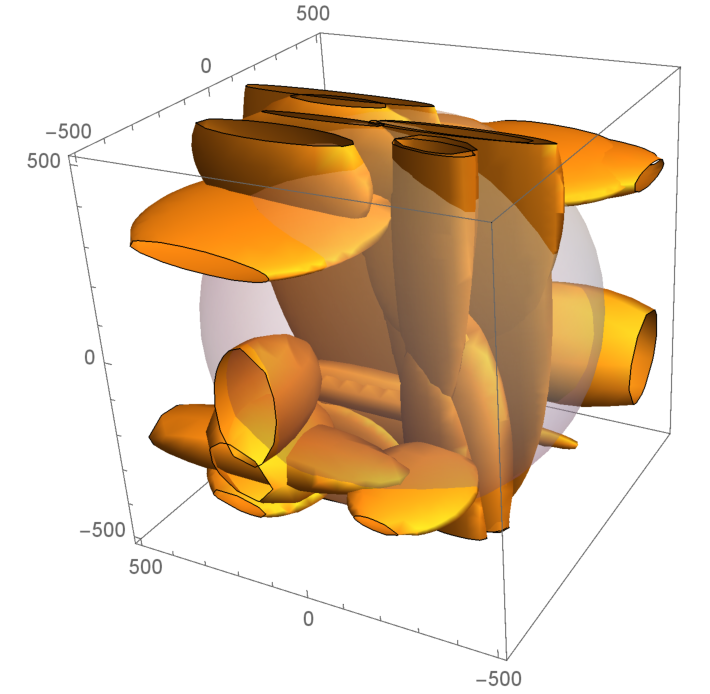
\includegraphics[width=0.9\textwidth]{./img/correlation3}
 \caption{Covariance tensor field for PI with deterministic (standard) algorithm - only the tensors with highest norm are presented}
\end{figure}

%\begin{figure}[h] 
% \centering \label{tennot}
% \includegraphics[width=0.9\textwidth]{../mathematica/nondet}
% \caption{Covariance tensor field for PI with non-deterministic algorithm - future simulations are required to confirm and explain the discrepancy}
%\end{figure}

The figure \ref{tendet} shows that the correlation tensor is represented by highly ellipsoidal surfaces and hence, the isotropy seems to be significantly violated. This can have several reasons. First, an obvious possibility is a mistake in the code, but after careful inspection and previous applications with reasonable outcomes, we believe this is not the case.

Another and the most plausible source of anisotropy is the limited size of the grid. Based on the theoretical analysis, we expect that (much) larger grids will produce more isotropic configurations. Anisotropy can also be attributed to the initial and boundary conditions on the sphere, which are isotropic only to extent allowed by the geometry of the lattice and the coarse-graining of the velocity field. This question is left for the future investigation.